%% 
%% Copyright 2019-2024 Elsevier Ltd
%% 
%% This file is part of the 'CAS Bundle'.
%% --------------------------------------
%% 
%% It may be distributed under the conditions of the LaTeX Project Public
%% License, either version 1.3c of this license or (at your option) any
%% later version.  The latest version of this license is in
%%    http://www.latex-project.org/lppl.txt
%% and version 1.3c or later is part of all distributions of LaTeX
%% version 1999/12/01 or later.
%% 
%% The list of all files belonging to the 'CAS Bundle' is
%% given in the file `manifest.txt'.
%% 
%% Template article for cas-sc documentclass for 
%% double column output.

\documentclass[a4paper,fleqn]{cas-sc}

% If the frontmatter runs over more than one page
% use the longmktitle option.

%\documentclass[a4paper,fleqn,longmktitle]{cas-sc}

%\usepackage[numbers]{natbib}
%\usepackage[authoryear]{natbib}
\usepackage[authoryear,longnamesfirst]{natbib}

\usepackage{algorithm}
\usepackage[noend]{algorithmic}
\usepackage{subcaption} 
\usepackage{enumitem}

%%%Author macros
\usepackage{amssymb}
\usepackage{xspace}

\newcommand{\even}          {\raisebox{0.3ex}{\scalebox{0.7}{$\bigcirc$}}\xspace}
\newcommand{\odd}           {\scalebox{0.9}{$\square$}\xspace}
\newcommand{\subeven}       {\raisebox{0.3ex}{\scalebox{0.5}{$\bigcirc$}}\xspace}
\newcommand{\subodd}        {\scalebox{0.6}{$\square$}\xspace}
\newcommand{\player}        {\mathsf{p}\xspace}
\newcommand{\opponent}      {\overline{\mathsf{p}}\xspace}

\newcommand{\wregularform}  {$\omega$-regular form\xspace}
\newcommand{\wregulargames} {$\omega$-regular games\xspace}
\newcommand{\noc}           {{\small\textsf{No\textit{-}Opponent\textit{-}Cycle}}\xspace}
\newcommand{\nocchecker}    {{\small\textsf{NOC\textit{-}Checker}}\xspace}
\newcommand{\noceager}      {{\small\textsf{NOC\textit{-}Eager}}\xspace}
\newcommand{\nocfilter}     {{\small\textsf{NOC\textit{-}Filter}}\xspace}
\newcommand{\nocmemo}       {{\small\textsf{NOC\textit{-}Memo}}\xspace}
\newcommand{\nocq}          {{\small\textsf{NOCQ}}\xspace}
\newcommand{\zra}           {{\small\textsf{ZRA}}\xspace}

% \newtheorem{definition}{Definition}
% \newtheorem{example}{Example}

% % Define MiniZinc syntax highlighting
% \lstdefinelanguage{MiniZinc}{
%   keywords={include, constraint, output, array, of, var, bool},
%   morekeywords={[2] set, int, float, string},
%   keywordstyle=\color{blue}\bfseries,
%   keywordstyle={[2]\color{teal}\bfseries},
%   sensitive=true,
%   comment=[l]{\%}, 
%   morecomment=[s]{/*}{*/},
%   commentstyle=\color{gray}\ttfamily,
%   stringstyle=\color{red}\ttfamily,
%   morestring=[b]",    % Defines double-quoted strings
%   morestring=[b]',    % Defines single-quoted strings  basicstyle=\ttfamily\small,
%   numberstyle=\tiny\color{gray},
%   numbers=left,
%   stepnumber=1,
%   breaklines=true,
%   showstringspaces=false,
%   frame=single,
%   tabsize=2,
%   basicstyle=\ttfamily\footnotesize
% }

% \lstset{
%     basicstyle=\small\ttfamily,
%     backgroundcolor=\color{gray!10},
%     frame=single,
%     framerule=0pt,
%     columns=fullflexible,
%     breaklines=true,
%     xleftmargin=0.5em,
%     xrightmargin=0.5em
% }
\def\tsc#1{\csdef{#1}{\textsc{\lowercase{#1}}\xspace}}
\tsc{WGM}
\tsc{QE}
%%%

% Uncomment and use as if needed
%\newtheorem{theorem}{Theorem}
%\newtheorem{lemma}[theorem]{Lemma}
%\newdefinition{rmk}{Remark}
%\newproof{pf}{Proof}
%\newproof{pot}{Proof of Theorem \ref{thm}}

\begin{document}
\let\WriteBookmarks\relax
\def\floatpagepagefraction{1}
\def\textpagefraction{.001}

% Short title
\shorttitle{}    

% Short author
\shortauthors{}  

% Main title of the paper
\title [mode = title]{A Constraint-base approach for solving\\
deterministic \wregulargames}  

% Title footnote mark
% eg: \tnotemark[1]
\tnotemark[1] 

% Title footnote 1.
% eg: \tnotetext[1]{Title footnote text}
\tnotetext[1]{} 

% First author
%
% Options: Use if required
% eg: \author[1,3]{Author Name}[type=editor,
%       style=chinese,
%       auid=000,
%       bioid=1,
%       prefix=Sir,
%       orcid=0000-0000-0000-0000,
%       facebook=<facebook id>,
%       twitter=<twitter id>,
%       linkedin=<linkedin id>,
%       gplus=<gplus id>]

\author[1]{}%[<options>]

% Corresponding author indication
\cormark[1]

% Footnote of the first author
\fnmark[1]

% Email id of the first author
\ead{}

% URL of the first author
\ead[url]{}

% Credit authorship
% eg: \credit{Conceptualization of this study, Methodology, Software}
\credit{}

% Address/affiliation
\affiliation[1]{organization={},
            addressline={}, 
            city={},
%          citysep={}, % Uncomment if no comma needed between city and postcode
            postcode={}, 
            state={},
            country={}}

\author[2]{}%[]

% Footnote of the second author
\fnmark[2]

% Email id of the second author
\ead{}

% URL of the second author
\ead[url]{}

% Credit authorship
\credit{}

% Address/affiliation
\affiliation[2]{organization={},
            addressline={}, 
            city={},
%          citysep={}, % Uncomment if no comma needed between city and postcode
            postcode={}, 
            state={},
            country={}}

% Corresponding author text
\cortext[1]{Corresponding author}

% Footnote text
\fntext[1]{}

% For a title note without a number/mark
%\nonumnote{}

% Here goes the abstract
\begin{abstract}
Solving \wregulargames is a core problem in formal verification, particularly within model checking and synthesis methods that have several industrial-scale applications. In this paper, we propose a constraint-based approach for games on graphs, built upon a novel propagation algorithm that eliminates opponent cycles from the game graph. This approach yields an efficient method that directly exploits the duality between players in a parity game. Our implementation within a Lazy Clause Generation framework outperforms all existing constraint-based methods for parity games. Furthermore, it performs competitively against the most specialized, non-CP-based algorithms---often matching and sometimes exceeding their performance---while retaining the inherent flexibility of general constraint-based approaches. 

Because new constraints can be seamlessly integrated, our method provides a highly flexible framework for refining existing problem formulations to search for preferred solutions. This extensibility allows the framework to solve multi-conditioned games, such as those combining parity conditions with cost or resource-bounded requirements. Finally, we present the theoretical foundations of our approach, a comprehensive experimental evaluation, and an analysis of different algorithmic variants.
\end{abstract}

% Use if graphical abstract is present
%\begin{graphicalabstract}
%\includegraphics{}
%\end{graphicalabstract}

% Research highlights
\begin{highlights}
\item 
\item 
\item 
\end{highlights}


% Keywords
% Each keyword is seperated by \sep
\begin{keywords}
Constraint programming  \sep Parity games \sep Verification.
\end{keywords}

\maketitle

\newpage
\tableofcontents
\newpage

\section{Introduction}
Two-player, zero-sum, infinite-duration games played on graphs provide the foundational mathematical framework for the automated verification and synthesis of reactive systems. In this paradigm, vertices represent states of the system and its environment, edges denote possible transitions or actions, and infinite paths (plays) represent the ongoing behaviour of the system. Solving these games—determining which player can force a play to satisfy a specific objective—is central to model checking, synthesis of controllers, and verifying specifications against adversarial environments.
%
Depending on the system requirements, these objectives are specified using different winning conditions on infinite paths. These are broadly categorized into qualitative and quantitative conditions. Qualitative conditions focus on the structural or topological properties of infinite paths; classic examples range from foundational objectives like reachability (visiting a target set of states at least once) and safety (remaining within a designated safe region indefinitely) to more complex $\omega$-regular specifications such as Büchi conditions (visiting designated states infinitely often) and parity conditions (evaluating the parity of the maximum priority seen infinitely often) \cite{Chatterjee:2012,Erich:2008}. Quantitative conditions, on the other hand, incorporate resource constraints or performance metrics, such as energy conditions (keeping a running resource counter above zero) and mean-payoff conditions (optimizing the long-run average reward)\cite{ChatterjeeHJ05,Chaloupka:2011}.
%
While specialized, highly tuned algorithms exist for isolated game types—most notably for parity games, which belong to $\mathsf{NP} \cap \mathsf{co\textit{-}NP}$~\cite{Jurdziński:1998}  —handling multi-conditioned objectives or transitioning between qualitative and quantitative variants often requires abandoning the underlying algorithmic machinery entirely. Because these state-of-the-art approaches rely on dedicated engines hardcoded to exploit the distinct mathematical structure of a single winning condition, they lack architectural modularity. Consequently, extending them to multi-conditioned settings typically requires complex reductions that fundamentally alter the game graph, leading to severe state-space explosion.
%
Traditional attempts to apply general combinatorial optimization frameworks, such as static reductions to Boolean Satisfiability (SAT), suffer from severe scalability bottlenecks. Forbidding winning cycles for an opponent via propositional logic leads to a massive explosion in formula size~\cite{Heljanko:2012}, severely limiting their practical application. In this paper, we overcome these limitations by presenting a unified, constraint-based approach capable of solving deterministic \wregulargames across a spectrum of winning conditions. Instead of relying on rigid, monolithic encodings, our approach is built upon a novel propagation algorithm designed to dynamically eliminate opponent winning cycles from the game graph. By abstracting the core graph reasoning into a dedicated constraint propagator, our method directly exploits the inherent duality between players, providing a symmetric and highly efficient mechanism for filtering invalid actions.
%
We implement this system within a Lazy Clause Generation (LCG) framework~\cite{DBLP:journals/constraints/OhrimenkoSC09}. By dynamically reasoning about the graph's structure during search and generating precise explanations for edge prunings, our framework combines the operational efficiency of specialized graph algorithms with the conflict-driven learning capabilities of modern constraint solvers. Empirical evaluations \cite{Hernandez:2026:noc} demonstrate that this approach not only outperforms previous constraint-based and SAT-based formulations for qualitative games like parity, but also performs highly competitively against state-of-the-art, non-CP-based specialized algorithms. More importantly, we show that the inherent flexibility of general constraint programming allows our framework to seamlessly scale from purely qualitative objectives (Büchi, parity) to complex quantitative settings (energy, mean-payoff), as well as multi-conditioned formulations where qualitative and quantitative constraints must be satisfied simultaneously.

The remainder of this paper is organized as follows. Section...
\todo{complete}

\section{Preliminaries}\label{sec:prelims}

%------------------------------------------------------------------------------

\subsection{Turn-Based Games on Graphs}
\label{sec:turn_based_games}

An \wregulargame is a two-player, zero-sum game of infinite duration played on a directed graph called an \textit{arena}. Two players, \textit{Even} (denoted as $\even$) and \textit{Odd} (denoted as $\odd$), move a token along adjacent vertices. The vertex where the token currently resides determines which player chooses the next transition. This ongoing process generates an infinite sequence of states. The ultimate winner of the game depends on whether this sequence satisfies a specific objective, defined by the game's winning condition.

\begin{definition}[Arena]\label{def:arena}
A turn-based game \textit{arena} $\mathcal{A}$ is a tuple $\mathcal{A} = (V, E, \Omega, \Xi)$, where:
\begin{itemize}
    \item $V$ is a finite set of vertices partitioned into two disjoint sets: $V_{\even}$ (vertices controlled by Player~$\even$) and $V_{\odd}$ (vertices controlled by Player~$\odd$).
    \item $E \subseteq V \times V$ is a set of directed transitions such that every vertex has at least one outgoing edge, i.e., $\forall v \in V, |vE| \geq 1$, where $vE = \{ w \in V \mid (v, w) \in E \}$ denotes the set of successors of $v$. We denote $Ev = \{ u \in V \mid (u, v) \in E \}$ as the set of predecessors of $v$.
    \item $\Omega: V \to \mathbb{N}$ is a priority colouring function that assigns to each vertex a non-negative integer priority (primarily utilized in qualitative contexts).
    \item $\Xi: E \to \mathbb{Z}$ is a weight function that assigns an integer weight to each transition, representing resource costs or rewards (primarily utilized in quantitative contexts).
\end{itemize}
\end{definition}

A game begins with a token placed at an initial vertex $v_0 \in V$. If $v_0 \in V_{\even}$, Player~$\even$ selects a successor $v_1 \in v_0E$; if $v_0 \in V_{\odd}$, Player~$\odd$ makes the selection. The token is then moved to $v_1$, and the process repeats indefinitely. This sequence of choices produces an infinite path $\pi = v_0 v_1 v_2 \ldots$ such that $(v_i, v_{i+1}) \in E$ for all $i \geq 0$, which is formally termed a \textit{play}. We denote the set of all infinite plays in $\mathcal{A}$ as $\text{Plays}(\mathcal{A})$. Given a play $\pi$, we define $\text{Inf}(\pi) \subseteq V$ as the set of vertices that appear infinitely often in $\pi$.

%------------------------------------------------------------------------------

\subsection{Strategies and Determinism}
A \textit{memoryless} strategy for Player~$\even$ is a function $\sigma: V_{\even} \to V$ such that $\sigma(v) \in vE$ for all $v \in V_{\even}$. Symmetrically, a memoryless strategy for Player~$\odd$ is a function $\tau: V_{\odd} \to V$ such that $\tau(v) \in vE$ for all $v \in V_{\odd}$. These strategies depend solely on the current position of the token, ignoring the history of the play. A pair of memoryless strategies $(\sigma, \tau)$ completely determines a unique infinite play $\pi(v_0, \sigma, \tau) = v_0 v_1 v_2 \ldots$ starting from a designated initial vertex $v_0 \in V$. 

An objective $\mathcal{W}$ for Player~$\even$ is a subset of all possible infinite plays, $\mathcal{W} \subseteq \text{Plays}(\mathcal{A})$. A strategy $\sigma$ is a winning strategy for Player~$\even$ from the initial vertex $v_0$ if, for all possible adversarial strategies $\tau$ of Player~$\odd$, the resulting unique play satisfies the objective, i.e., $\pi(v_0, \sigma, \tau) \in \mathcal{W}$. Due to the memoryless determinism of the deterministic \wregulargames\ studied here~\cite{Zielonka:1998}, if a player has a winning strategy from $v_0$, they are guaranteed to have a memoryless one. 

In this work, we focus on the \textit{initial-vertex game solving problem}. Given a game arena $\mathcal{A}$ and a specific starting vertex $v_0 \in V$, the goal is to determine which of the two players has a winning strategy starting from $v_0$, and to construct that specific winning strategy.

%------------------------------------------------------------------------------

\subsection{Winning Conditions for \wregulargames}
\label{sec:winning_conditions}

The classification of an infinite play as winning or losing is governed by the game's \textit{winning condition}, which dictates how the path's structural or numerical properties are evaluated. From a player's perspective, this condition defines their \textit{objective} $\mathcal{W} \subseteq \text{Plays}(\mathcal{A})$, representing the specific set of plays they aim to enforce. For consistency across all discussed variants, we focus on the objective $\mathcal{W}$ from the perspective of Player~$\even$. Because these games are zero-sum, a play $\pi$ is winning for Player~$\even$ if $\pi \in \mathcal{W}$, and winning for Player~$\odd$ if $\pi \notin \mathcal{W}$. 

We partition these objectives into two major paradigms: \textit{qualitative conditions}, which evaluate the structural topology of the vertices visited infinitely often (or reached within a finite horizon), and \textit{quantitative conditions}, which evaluate the numerical accumulation of resource weights along the traversed edges.

\subsubsection{Qualitative Conditions}
\label{subsec:qualitative}

Qualitative conditions depend strictly on the set of vertices that appear infinitely often in a play $\pi$, denoted as $\text{Inf}(\pi) \subseteq V$. While our core framework addresses complex $\omega$-regular behaviors defined over these infinite limits, it inherently scales down to foundational, finite-horizon qualitative properties. Specifically, \textit{Reachability} objectives require Player~$\even$ to hit a target set $T \subseteq V$ at least once along the play, whereas \textit{Safety} objectives demand that the play remains entirely within a designated safe region $S \subseteq V$ indefinitely. Beyond these basic properties, we focus on the following standard $\omega$-regular qualitative conditions:

\paragraph{Büchi Objectives:}
A Büchi condition is defined relative to a designated set of target vertices $F \subseteq V$. The objective for Player~$\even$ is to visit this set infinitely often. Formally, a play $\pi$ satisfies the Büchi objective if $\text{Inf}(\pi) \cap F \neq \emptyset$.
Conversely, the dual co-Büchi objective requires that the play eventually settles outside the complement of $F$, meaning that vertices outside $F$ are visited only finitely many times. A play $\pi$ satisfies the co-Büchi objective if $\text{Inf}(\pi) \subseteq F$.

\paragraph{Parity Objectives:}
The parity condition evaluates a play using the arena's priority colouring function $\Omega: V \to \mathbb{N}$. Player~$\even$ satisfies the parity objective if the maximum priority that appears infinitely often along the play is an even integer.
\[
\max \{ \Omega(v) \mid v \in \text{Inf}(\pi) \} \bmod 2 = 0 
\]

Conversely, if this maximum priority is an odd integer, the play is won by Player~$\odd$.

\subsubsection{Quantitative Conditions}
\label{subsec:quantitative}

Quantitative conditions shift the evaluation to the infinite sequence of transitions $e_0 e_1 e_2 \ldots$ generated during a play $\pi = v_0 v_1 v_2 \ldots$, tracking numerical behaviours via the arena's edge weight function $\Xi: E \to \mathbb{Z}$.

\paragraph{Energy Objectives:}
Energy conditions model games with physical resource constraints, where Player~$\even$ must navigate the arena indefinitely without ever allowing the resource level to drop below zero. Under memoryless strategies, any infinite play $\pi$ eventually settles into a closed terminal cycle. Consequently, satisfying the energy objective is equivalent to ensuring that the net resource change over this loop is non-negative, preventing a systematic depletion of the resource over time. Formally, letting $E' \subseteq E$ denote the set of directed transitions comprising this terminal cycle, Player~$\even$ satisfies the objective if the accumulated weights of the edges in the loop meet or exceed a designated threshold $\nu \in \mathbb{Z}$ (typically $\nu = 0$):
\[
\sum_{(v, w) \in E'} \Xi(v, w) \geq \nu
\]

\paragraph{Mean-Payoff Objectives:}
Mean-payoff conditions evaluate the long-term average reward or cost accumulated per transition over an infinite duration. Under memoryless strategies, any infinite play $\pi$ eventually settles into a closed terminal cycle, meaning the long-run performance is entirely determined by the transitions repeated within this loop. Consequently, satisfying the mean-payoff objective is equivalent to ensuring that the average edge weight over this cycle meets or exceeds a specified threshold. Formally, letting $E' \subseteq E$ denote the set of directed transitions comprising this terminal cycle, Player~$\even$ satisfies the objective if the average weight of the edges in this subset meets or exceeds a designated performance threshold $\nu \in \mathbb{R}$:
\[
\frac{1}{|E'|} \sum_{(v, w) \in E'} \Xi(v, w) \geq \nu
\]

%------------------------------------------------------------------------------

\subsection{Constraint Programming and Propositional Satisfiability}
\todo{Introduce CP and SAT}

% \section{Constraint Programming Framework for Game Solving}\label{sec:cp_framework}
% \subsection{Decision Variables and Local Strategy Characterization}\label{sec:variables_local}
% \subsection{Baseline Formulation: Monolithic SAT Encoding}\label{sec:sat_baseline}

%==============================================================================

\section{Constraint Programming Framework for Game Solving}
\label{sec:cp_framework}

This section describes our constraint programming (CP) framework for solving deterministic \wregulargames\ from an initial-vertex perspective. We first formalize how local memoryless strategies are characterized via Boolean decision variables. We then outline the traditional monolithic SAT/SMT baseline formulation to highlight the structural and scalability challenges that motivate our unified global propagator approach.

%------------------------------------------------------------------------------

\subsection{Decision Variables and Local Strategy Characterization}
\label{sec:variables_local}

To solve an initial-vertex game using a constraint-based approach, the search space for a winning memoryless strategy must be mapped into finite-domain decision variables. 
%
Let $\player \in \{\even, \odd\}$ denote the \textit{player of interest}, and let $\opponent$ represent their designated opponent, defined as:

$\opponent = \begin{cases} \even & \text{if } \player = \odd, \\ \odd & \text{if } \player = \even. \end{cases}$

We partition the finite set of vertices $V$ of the arena $\mathcal{A}$ into $V_{\player}$ (vertices controlled by the player of interest) and $V_{\opponent}$ (vertices controlled by the opponent). 

Given a specific starting vertex $v_0 \in V$, we introduce two sets of Boolean decision variables to track the active sub-graph induced by the players' strategic choices during the search:
\begin{itemize}
    \item $\mathcal{V}_v \in \{\top, \bot\}$ for each vertex $v \in V$, denoting whether vertex $v$ is reachable from $v_0$ under the currently explored strategy profile.
    \item $\mathcal{E}_e \in \{\top, \bot\}$ for each directed edge $e \in E$, denoting whether transition $e$ is actively selected or traversed within the strategy sub-graph.
\end{itemize}

The structural conditions required to characterize a valid winning play from $v_0$ for the player of interest are deeply rooted in the classic game-theoretic concept of an \textit{attractor}. Given a target set of vertices, the $\player$-attractor is the set of states from which $\player$ can force the play into that target set in a finite number of steps, regardless of the choices made by $\opponent$. ~\cite{Zielonka:1998,Aggarwal:2023}. 

To embed this operational capability natively into our CP variable framework, the active strategy sub-graph must be constrained such that $\player$ maintains absolute deterministic control, while simultaneously guarding against every possible counter-move from $\opponent$. Structurally, this requires enforcing the following connectivity rules from $v_0$:
\begin{itemize}
    \item \textbf{Root Activation:} The initial vertex must always be active ($\mathcal{V}_{v_0} = \top$).
    \item \textbf{Deterministic Selection:} For every active vertex controlled by the player of interest ($v \in V_{\player}$), the solver must select one outgoing transition to enforce a positional choice.
    \item \textbf{Adversarial Closure:} For every active vertex controlled by the opponent ($v \in V_{\opponent}$), the formulation must activate \textit{all} of its outgoing transitions. This models the attractor logic by guaranteeing that no matter which edge the opponent selects, the play cannot escape the verified strategy graph.
    \item \textbf{Forward Propagation:} Any vertex reached by an active edge must itself be marked as active.
\end{itemize}

By combining these structural layout constraints, the CP solver isolates a well-formed sub-arena where Player~$\player$ has a valid strategy from $v_0$. The remaining task for the solver is to ensure that the cycles formed within this attractor structure satisfy the designated qualitative or quantitative winning conditions.

\begin{itemize}
    \item \textbf{Winning Evaluation:} The active sub-graph must guarantee that any infinite path originating from $v_0$ satisfies the specific winning conditions established in Section~\ref{sec:winning_conditions}. Operationally, the solver imposes structural or numerical constraints to ensure that all active cycles conform to these criteria, preventing the opponent from forcing the play into a losing infinite loop.
\end{itemize}

%------------------------------------------------------------------------------

\subsection{Baseline Formulations and the Generalized CSP Model}
\label{sec:sat_baseline}

Historically, constraint-based game solving has relied on encoding cycle conditions statically into propositional logic. The standard reference approach by Heljanko et al.~\cite{Heljanko:2012} translates a game into Boolean Satisfiability (SAT) or Satisfiability Modulo Theories (SMT) formulas by leveraging a \textit{progress measure}~\cite{Jurdziński:2000}.

In this baseline formulation, the structural graph properties are captured by the following difference logic formula straightforward to reduce to a Conjunctive Normal Form (CNF):
\begin{itemize}
    \item $\Phi_\exists = \bigwedge_{v \in V_{\subeven}} \left(S_v \rightarrow \bigvee_{w \in vE} T_{(v,w)}\right)$
    \item $\Phi_\forall = \bigwedge_{v \in V_{\subodd}} \left(S_v \rightarrow \bigwedge_{w \in vE} T_{(v,w)}\right)$
    \item $\Phi_V = \bigwedge_{w \in V, w \neq v_0} \left( \left(\bigvee_{v \in Ev} T_{(v,w)}\right) \rightarrow S_w \right)$
\end{itemize}
where $S_v$ and $T_{(v,w)}$ are Boolean variables tracking the winning paths for Player~$\even$. 
%
To enforce the parity condition along infinite paths, additional integer variables $x_p^v$ are introduced for every vertex $v$ and every odd priority $p \in \textit{Odd}(G)$. These variables track numerical progress along active transitions via difference logic constraints ($\Phi_A$):


To enforce the parity condition along infinite paths, additional integer variables $x_p^v$ are introduced for every vertex $v \in V$ and every odd priority $p \in \textit{Odd}(G)$, where $\textit{Odd}(G) = \{ p \in \mathbb{N} \mid p \pmod 2 \neq 0 \land \exists v \in V: \Omega(v) = p \}$ represents the set of all odd priorities present in the arena. These variables track numerical progress along active transitions via difference logic constraints ($\Phi_A$):

\begin{itemize}
    \item $\Phi_A = \bigwedge_{(v,w) \in E} \left(T_{(v,w)} \rightarrow \Psi_{(v,w)}\right)$
    \item $\Psi_{(v,w)} = \bigwedge_{p \in \textit{Odd}^{>\Omega(w)}(G)} (x_p^v \geqslant x_p^w), \quad \text{if } \Omega(w) \text{ is even}$
    \item $\Psi_{(v,w)} = \bigwedge_{p \in \textit{Odd}^{>\Omega(w)}(G)} (x_p^v \geqslant x_p^w) \land (x_{\Omega(w)}^v > x_{\Omega(w)}^w), \quad \text{if } \Omega(w) \text{ is odd}$
\end{itemize}
These difference logic assertions force a strict mathematical contradiction (such as $x_p^v > x_p^v$) along any active cycle dominated by an odd priority. This renders the system of constraints logically unsatisfiable along that specific path, structurally forcing the solver's backtracking engine to reject assignments containing odd-winning loops and isolate only even-winning cycles.

The fundamental principle of this constraint-based approach is to reduce game-theoretic determinacy to propositional satisfiability. Determining the satisfiability of the combined formula $(S_{v_0} \wedge \Phi_{\exists} \wedge \Phi_{\forall} \wedge \Phi_V \wedge \Phi_A)$ is equivalent to deciding the winner of the game. A satisfying assignment serves as a constructive proof that Player~\even\ has a winning strategy from $v_0$. Conversely, because the encoding completely characterizes Player~\even's winning conditions, an exhaustive proof of unsatisfiability establishes that no such strategy exists, which—by the determinacy of these games—constitutes a definitive proof of a win for Player~\odd.

\subsubsection{Limitations of the Monolithic Baseline}
While highly effective for pure parity games on small arenas, this monolithic encoding faces severe scaling and architectural bottlenecks when generalized to broader $\omega$-regular contexts:
\begin{enumerate}
     \item \textbf{Space and Formula Explosion:} In terms of static allocation space, the method requires instantiating $\mathcal{O}(|V| \cdot |\textit{Odd}(G)|)$ auxiliary variables and generating $\mathcal{O}(|E| \cdot |\textit{Odd}(G)|)$ difference logic constraints. For dense graphs with rich priority profiles, this upfront space requirement grows up to $\mathcal{O}(|V|^3)$. Crucially, this footprint escalates even further when the formulation is reduced to pure SAT solving. Converting the underlying integer difference logic into pure CNF requires bit-blasting or explicit circuit encodings for every inequality, multiplying the clause count and injecting hundreds of millions of literal allocations before the search even begins.
    \item \textbf{Inflexibility to Multi-Objectives:} Adapting progress measures to quantitative metrics (like energy levels or long-run averages) requires fundamentally reconstructing the underlying arithmetic variable layers, destroying the modularity of the framework.
\end{enumerate}

To overcome these structural limitations, we replace the entire monolithic CNF formula—including both the static graph connectivity clauses and the progress measure variables—with a unified, high-level Constraint Satisfaction Problem (CSP) abstraction. Instead of flattening the game's rules into a rigid propositional grid, this CP model captures the graph's topology natively through clean domain variables, while seamlessly handling arbitrary, multi-conditioned $\omega$-regular properties by delegating all cycle validation to a dynamic global propagator.

\begin{definition}[Generalized Game CSP]\label{def:csp}
The CSP for an arena $\mathcal{A} = (V, E, \Omega, \Xi)$ starting at an initial vertex $v_0$ from the perspective of Player~$\player$ is defined as the triple $\mathcal{P} = (\mathcal{X}, \mathcal{D}, \mathcal{C})$, where $\mathcal{X} = \{ \mathcal{V}_v \}_{v \in V} \cup \{ \mathcal{E}_e \}_{e \in E}$ represents the set of Boolean decision variables mapped to domains $\mathcal{D} = \{\bot, \top\}$, and $\mathcal{C}$ is the set of constraints defined by:
\begin{itemize}
    [leftmargin=2.3cm, labelwidth=2.8cm, align=right, itemsep=1.0ex, parsep=0pt]
    \item [$\mathcal{C}_{v_0}$ :] $\mathcal{V}_{v_0} = \top$
    \item [$\mathcal{C}_{\player}$ :] $\bigwedge_{v \in V_{\player}} \left(\mathcal{V}_v \rightarrow \left(\sum_{w \in vE} \mathcal{E}_{(v,w)}= 1\right)\right)$
    \item [$\mathcal{C}_{\opponent}$ :] $\bigwedge_{v \in V_{\opponent}} \left(\mathcal{V}_v \rightarrow \bigwedge_{w \in vE} \mathcal{E}_{(v,w)}\right)$
    \item [$\mathcal{C}_{\!E}$ :] $\bigwedge_{w \in V, w \neq v_0} \left(\left(\bigvee_{v \in Ew} \mathcal{E}_{(v,w)}\right) \rightarrow \mathcal{V}_w\right)$
    \item [$\mathcal{C}_{\noc}(f)$ :] $\bigwedge_{v_0, \closerdots, v_k} \left( \left(\bigwedge_{i=0}^{k-1} \mathcal{E}_{(v_i,v_{i+1})}\right) \to \bigwedge_{j=0}^{k-1} \left((v_j = v_k) \to f(v_j, \closerdots, v_k)\right) \right)$
\end{itemize}
where the evaluation criteria $f$ for a given cycle $v_j, \dots, v_k$ are provided by specific qualitative or quantitative verification functions—encompassing Büchi ($f^\mathcal{\varphi}$), Parity ($f^\omega$), Energy ($f^\eta$), and Mean-Payoff ($f^\mu$) conditions—which are formally detailed in Section~\ref{sec:function_conditions}.

\end{definition}

While constraints $\mathcal{C}_{v_0}$, $\mathcal{C}_{\opponent}$, and $\mathcal{C}_{\!E}$ enforce the required sub-graph connectivity (analogous to the baseline's $\Phi_{v_0}, \Phi_\forall$, and $\Phi_V$), $\mathcal{C}_{\player}$ strictly dictates that the protagonist selects exactly one deterministic strategy choice per active vertex. 

Crucially, our approach removes the expensive difference logic constraints $\Phi_A$ entirely. Instead, the global constraint $\mathcal{C}_{\noc}(f)$ monitors the strategy graph dynamically during the CP search loop. It intercepts any emerging path profile and applies a parameterized verification function $f$ to ensure that no reachable closed component is structurally and strategically winning for $\opponent$. Accordingly, we name our method \nocq, which stands for \nooppc with Qualitative and Quantitative conditions. The precise operational formulations for these qualitative and quantitative cycle evaluation functions are detailed thoroughly in Section~\ref{sec:function_conditions}.

Our generalized CSP model inherits and extends this satisfiability approach, lifting it from a fixed perspective to a modular framework. The semantic mapping between the satisfiability of the CSP and the game-theoretic outcome remains definitive: a satisfying assignment found by the solver proves that the player of interest, $\player$, possesses a positional winning strategy from $v_0$, where the active edges ($\mathcal{E}_e = \top$) map directly to their winning choices. 

A key architectural advantage of this design is that by simply swapping the roles of $\player$ and $\opponent$, the formulation allows the proposed method to search from the perspective of either player natively. While a satisfying assignment validates a win for $\player$, an exhaustive proof of unsatisfiability demonstrates the complete absence of a positional winning strategy for them, which—by the determinacy of these games—automatically hands a conclusive victory to the opponent $\opponent$.

%------------------------------------------------------------------------------

\subsection*{Example 1}
\label{sec:example1}

\begin{figure}
     \centering
     \makebox[\textwidth][c]{
         \begin{subfigure}[t]{0.51\textwidth}
             \centering
             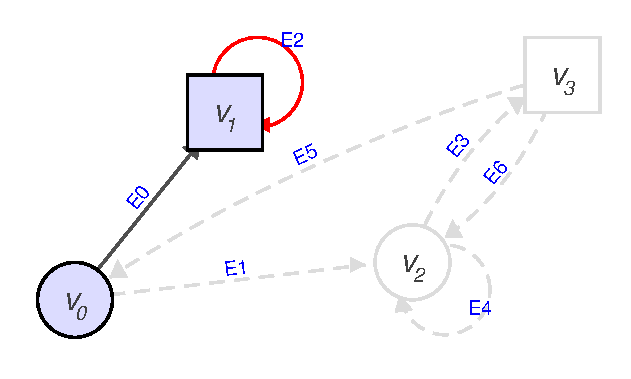
\includegraphics[width=0.8\textwidth, trim={0 0 0 0}, clip]{images/ex11.pdf}
             \vspace{-5pt}
             \caption{First assignment.}
             \label{fig:ex11}
         \end{subfigure}
         \hspace{1pt}
         \begin{subfigure}[t]{0.51\textwidth}
             \centering
             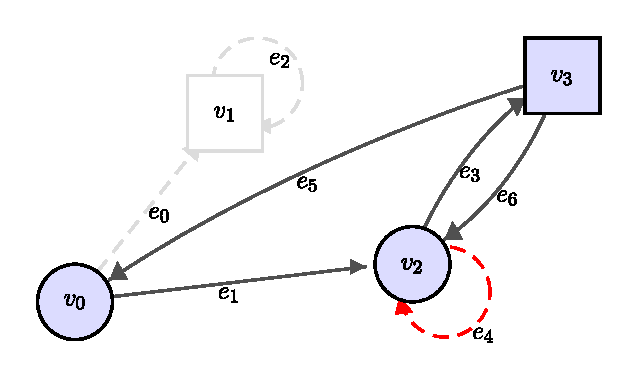
\includegraphics[width=0.8\textwidth, trim={0 0 0 0}, clip]{images/ex12.pdf}
             \vspace{-5pt}
             \caption{Second assignment}
             \label{fig:ex12}
         \end{subfigure}
     }
    \caption{Game arena featuring $|V|=4$ and $|E|=7$. Vertices in $V_{\even}$ are depicted as circles, and vertices in $V_{\odd}$ as squares. Active components are highlighted in solid black, unassigned/inactive elements are faded in gray or dashed lines, and red indicates a cycle rejected by the propagator.}     
    \label{fig:ex10}
\end{figure}

To demonstrate the structural and operational mechanics of our generalized CSP formulation, consider the 2-player game arena illustrated in Figure~\ref{fig:ex10}. The arena consists of four vertices $V = \{v_0, v_1, v_2, v_3\}$, which are partitioned into $V_{\even} = \{v_0, v_2\}$ and $V_{\odd} = \{v_1, v_3\}$. The directed edge set is defined as $E = \{e_0, e_1, e_2, e_3, e_4, e_5, e_6 \}$. We evaluate a Büchi objective from the perspective of Player~$\even$ ($\player = \even$), where the target accepting set is $F = \{v_3\}$, and the initial vertex is $v_0$.

Under our framework, the solver instantiates the following core set of Boolean decision variables:
\[
\mathcal{X} = \{\mathcal{V}_0, \mathcal{V}_1, \mathcal{V}_2, \mathcal{V}_3, \mathcal{E}_0, \mathcal{E}_1, \mathcal{E}_2, \mathcal{E}_3, \mathcal{E}_4, \mathcal{E}_5, \mathcal{E}_6 \}.
\]
 
The structural constraints $\mathcal{C}_{v_0}$, $\mathcal{C}_{\player}$, $\mathcal{C}_E$, and $\mathcal{C}_{\opponent}$ allow the solver to make an initial assignment activating $\mathcal{V}_0, \mathcal{E}_0, \mathcal{V}_1$, and $\mathcal{E}_2$ by setting these variables to $\top$ (see Figure~\ref{fig:ex11}). At this stage, the global constraint $\mathcal{C}_{\noc}$ determines the existence of a unique cycle:

\begin{itemize}
    \item \textbf{Cycle ($v_1 \rightarrow v_1$):} Traversing the self-loop edge $e_2$, the solver evaluates the cycle sequence:
    \[
    f^\mathcal{\varphi}(v_1, v_1) = \{v_1\} \cap \{v_3\} = \emptyset \implies \bot.
    \]
\end{itemize}

The propagator immediately rejects this branch because the infinite path trapped in this cycle fails the Büchi condition, forcing the solver to backtrack. 

In a subsequent alternative assignment, the structural constraints activate the variables $\mathcal{V}_0, \mathcal{E}_1, \mathcal{V}_2, \mathcal{E}_3, \mathcal{V}_3, \mathcal{E}_5$, and $\mathcal{E}_6$ by setting them to $\top$ (see Figure~\ref{fig:ex12}). At this point, the structural layout constraints have successfully isolated a valid candidate strategy sub-graph. The global constraint $\mathcal{C}_{\noc}(f^\mathcal{\varphi})$ scans this active sub-arena and extracts all reachable loops to evaluate their infinite behavior against the Büchi conditions:

\begin{itemize}
    \item \textbf{Cycle ($v_0 \rightarrow v_2 \rightarrow v_3 \rightarrow v_0$):} Traversing edges $e_1, e_3$, and $e_5$, the solver evaluates the cycle sequence:
    \[
    f^\mathcal{\varphi}(v_0, v_2, v_3, v_0) = \{v_0, v_2, v_3\} \cap \{v_3\} \neq \emptyset \implies \top.
    \]
    \item \textbf{Cycle ($v_2 \rightarrow v_3 \rightarrow v_2$):} Reachable via $e_1$ and traversing edges $e_3$ and $e_6$, the solver evaluates the tighter internal loop:
    \[
    f^\mathcal{\varphi}(v_2, v_3, v_2) = \{v_2, v_3\} \cap \{v_3\} \neq \emptyset \implies \top.
    \]
\end{itemize}

Because every active cycle within this adversarial sub-graph contains a vertex from the accepting set $F$, any resulting infinite path satisfies the winning criteria. The global constraint validates the assignment, and the solver successfully terminates, outputting a satisfying assignment that proves Player~$\even$ wins the game from $v_0$.


%------------------------------------------------------------------------------

\subsection{Global Opponent Cycle Elimination Propagators}
\label{sec:global_propagators}

Before detailing the inner workings of our cycle elimination algorithms, it is important to clarify how the different components of the generalized Game CSP (Definition~\ref{def:csp}) are implemented within the underlying solver. The localized structural constraints—namely the root activation ($\mathcal{C}_{v_0}$), the player's deterministic choice ($\mathcal{C}_{\player}$), the opponent's attractor expansion ($\mathcal{C}_{\opponent}$), and the forward edge propagation ($\mathcal{C}_E$)—consist of simple, local logical dependencies. Consequently, they are mapped directly to standard propositional clauses or native primitive constraints managed efficiently by the solver's default propagation engine. 

In contrast, the cycle validation constraint $\mathcal{C}_{\noc}(f)$ governs non-local, dynamic graph properties that cannot be captured effectively by static clauses. This necessitates the introduction of a custom, highly specialized global propagator to monitor the emerging strategy graph and dynamically prune illegal loops during search.

To dynamically enforce the global constraint $\mathcal{C}_{\noc}(f)$ during the search loop, we introduce three algorithmic variants designed to intercept, analyze, and eliminate illegal winning components for the opponent $\opponent$. Rather than relying on rigid, upfront propositional expansions, these propagators run natively inside the CP solver's execution engine, providing varying trade-offs between filtering strength and algorithmic complexity.


Before detailing the inner workings of our cycle elimination algorithms, it is important to clarify how the different components of the generalized Game CSP (Definition~\ref{def:csp}) are implemented within the underlying solver. The localized structural constraints—namely the root activation ($\mathcal{C}_{v_0}$), the player's deterministic choice ($\mathcal{C}_{\player}$), the opponent's attractor expansion ($\mathcal{C}_{\opponent}$), and the forward edge propagation ($\mathcal{C}_E$)—consist of simple, local logical dependencies. Consequently, they are mapped directly to standard propositional clauses or native primitive constraints managed efficiently by the solver's default propagation engine. In our 

In contrast, the cycle validation constraint $\mathcal{C}_{\noc}(f)$ governs non-local, dynamic graph properties that cannot be captured effectively by static clauses. This necessitates the introduction of a custom, highly specialized global propagator to monitor the emerging strategy graph and dynamically prune illegal loops during search.

To make this global propagator fully modular across multi-conditioned arenas, we decouple the global path evaluation function $f$ into an abstract, vertex-level winning predicate. We define the global objective profile as a conjunctive operator composition over the individual game criteria:
\[
f = f^\mathcal{\varphi} \otimes f^\omega \otimes f^\eta \otimes f^\mu 
\]
where $\varphi, \omega, \eta$, and $\mu$ represent qualitative and quantitative objectives (specifically Büchi, parity, energy boundaries, and mean-payoffs, respectively). 

Correspondingly, for any individual state, the predicate $f_{\player}(v)$ evaluates whether the local property of vertex $v$ satisfies or actively contributes to the winning requirements of $\player$ under the composed objective $f_{\player}$. If $f_{\player}(v)$ holds true, vertex $v$ belongs to the safe region for the player of interest; if false ($\neg f_{\player}(v)$), the state inherently risks driving the game into a component dominated by the adversary. The algorithms in this section leverage this predicate to systematically slice away valid sub-graphs and isolate losing loops.

\subsubsection{A No-Opponent-Cycle Checker  (\nocchecker)} \label{sec:nocchecker}

Our first baseline propagator establishes a fundamental validation check by recursively decomposing the strategy sub-graph into Strongly Connected Components (SCCs). By definition, every vertex inside an SCC of cardinality greater than one belongs to at least one localized cycle, whereas single-vertex SCCs can only close a loop via an explicit self-loop. 

The checker isolates the induced active sub-graph containing only assigned variables where $\mathcal{V}_v = \top$ and $\mathcal{E}_e = \top$. It then systematically identifies and eliminates vertices that satisfy the winning condition for $\player$, checking whether any residual components form an inescapable cycle that exclusively favors $\opponent$.

\begin{algorithm}[htb]
\small
\caption{\textbf{\nocchecker}}
\textbf{Input}: Induced active sub-graph $G = (V', E')$ \\
\textbf{Output}: $\top$ if the strategy graph contains no winning opponent cycles; $\bot$ otherwise
\begin{algorithmic}[1]
    \FOR{$scc \in \textit{Tarjan}(G)$} \label{alg:nocchecker:breakingdown}
        \IF{$|scc| = 1$} \label{alg:nocchecker:single}
            \STATE $v \gets$ the unique vertex in $scc$
            \STATE \textbf{if } $\neg f_{\player}(v) \land \mathcal{E}_{[vEv]}$ \textbf{then return $\bot$} \label{alg:nocchecker:self}  
        \ELSE
            \STATE $ \textit{objectiveSet} \gets \{ v \in scc \mid 
            f_{\player}(v) \text{ holds true}
            \}$ \label{alg:nocchecker:best}
            \STATE \textbf{if } $ \textit{objectiveSet} = \emptyset$ \textbf{then return $\bot$} \label{alg:nocchecker:opponent}

            \STATE \nocchecker($G \setminus \textit{objectiveSet}$) \label{alg:nocchecker:recursion}
        \ENDIF
    \ENDFOR
    \RETURN $\top$
\end{algorithmic}
\label{alg:nocchecker}
\end{algorithm}

\begin{algorithm}[htb]
\small
\caption{\textbf{\nocchecker-Qt}}
\textbf{Input}:  Induced active sub-graph $G = (V', E')$,
                 threshold $\nu \in \mathbb{Z}$ \\
\textbf{Output}: $\top$ if the strategy graph contains no winning opponent cycles;
                 $\bot$ otherwise
\begin{algorithmic}[1]
    \FOR{$\textit{scc} \in \textit{Tarjan}(G)$}
    \label{alg:nocqt:tarjan}
        \IF{$|\textit{scc}| = 1$}
        \label{alg:nocqt:single}
            \STATE $v \gets$ the unique vertex in $\textit{scc}$
            \IF{$\mathcal{E}_{[vEv]} $}
            \label{alg:nocqt:selfloop}
                \STATE \textbf{if } $\Xi(v,v) < \nu$
                       \textbf{ then return } $\bot$
                \label{alg:nocqt:selfenergy}
            \ENDIF
        \ELSE
            \IF{$f^{\eta}$ \textbf{ and }
                $\textit{MinEnergyCycle}(\textit{scc}) < 0$}
            \label{alg:nocqt:energy}
                \RETURN $\bot$
            \ENDIF
            \IF{$f^{\mu}$ \textbf{ and }
                $\textit{MinMeanCycle}(\textit{scc},\,\nu)$}
            \label{alg:nocqt:mean}
                \RETURN $\bot$
            \ENDIF
        \ENDIF
    \ENDFOR
    \RETURN $\top$
\end{algorithmic}
\label{alg:noccheckerQuant}
\end{algorithm}

Algorithm~\ref{alg:nocchecker} is executed when all decision variables within the current search branch become fixed. The function is invoked with the induced sub-graph containing exclusively the active components: \nocchecker$(\{ v \in V \mid \mathcal{V}_v = \top \})$.

The graph is first partitioned into independent components using Tarjan's linear-time algorithm (Line~\ref{alg:nocchecker:breakingdown}). If an SCC contains an isolated vertex (Line~\ref{alg:nocchecker:single}), the algorithm ensures it does not possess an active self-loop ($\mathcal{E}_{[vEv]} = \top$) that violates the evaluation predicate $f_{\player}(v)$ (Line~\ref{alg:nocchecker:self}). For non-trivial components, the algorithm isolates the subset of vertices that satisfy the winning criteria for the player of interest: $\textit{objectiveSet} \gets \{ v \in scc \mid f_{\player}(v) \}$ (Line~\ref{alg:nocchecker:best}). 

If this filtering step yields an empty set ($\textit{objectiveSet} = \emptyset$), it mathematically demonstrates that the entire component forms a closed cycle where no state can satisfy the winning criteria for $\player$ (Line~\ref{alg:nocchecker:opponent}). Due to the structural nature of these games, this represents an inescapable loop favoring the adversary, and the assignment is rejected. Otherwise, if the set is not empty, those validated states are filtered out, and the checker is recursively called on the remaining induced sub-graph ($G \setminus \textit{objectiveSet}$) to ensure that no secondary, losing sub-cycles are nested within the component (Line~\ref{alg:nocchecker:recursion}).

The worst-case computational complexity of \nocchecker remains strictly polynomial. A single pass of Tarjan’s algorithm runs in linear time $\mathcal{O}(|V| + |E|)$. Because vertices within the valid objective sets are removed permanently at each recursive tier, the maximal depth of the recursion is bounded linearly by the total number of vertices. Consequently, the overall time complexity of the checker stands at $\mathcal{O}(|V| \cdot (|V| + |E|))$ in the absolute worst case.

\subsubsection{A No-Opponent-Cycle Filter (\noceager)} \label{sec:nocfilter}

While the checker functions as a final validation step on fully assigned branches, proactive pruning requires an eager filtering mechanism. We propose a look-ahead propagator driven by a Depth-First Search (DFS) traversal. Rather than waiting for a complete assignment, this variant explores potential paths from the initial vertex $v_0$ to detect emerging cycles early. We formalize this algorithm within the context of a \textit{Lazy Clause Generation} (LCG) solver architecture, enabling the propagator to dynamically deduce and register learned propositional explanations when conflicts are reached.

\begin{algorithm}[htb]
\small
\caption{\textbf{\noceager}}
\textbf{Input}: $path_V,\ path_E,\ v,\ e,\ \mathcal{E},\ \textit{defined}$ \\
\textbf{Output}: $\top$ if look-ahead is valid; $\bot$ if a fatal conflict occurs
\begin{algorithmic}[1]
    \IF{$v \in path_V$} \label{alg:noceager:pathcheck}
        \STATE $i_v \gets \textit{find}(v, path_V)$ \label{alg:noceager:findcycle}
        \IF{$\neg f_{\player}(path_E[i_v:])$} \label{alg:noceager:checkopponent}
            \STATE $\textit{reason} \gets \textit{clausify}(\neg path_E)$ \label{alg:noceager:reason}
            \STATE \textbf{if } not $(\mathcal{E}_e \gets (\bot, \textit{reason}))$ \textbf{then return $\bot$}
        \ENDIF
    \ELSIF{$\textit{defined}$} \label{alg:noceager:defcheck}
        \FOR{$e' \in \textit{edges}(v) \textbf{ where } \mathcal{E}_{e'} \ne \bot$} \label{alg:noceager:edgecheck}
            \STATE $p_V \gets path_V \cup \{v\}$
            \STATE $p_E \gets path_E \cup \{e'\}$
            \STATE $w \gets \textit{target}(e')$
            \STATE $\textit{def} \gets (\mathcal{E}_{e'} = \top)$
            \STATE \noceager($p_V$, $p_E$, $w$, $e'$, $\mathcal{E}$, $\textit{def}$)
        \ENDFOR
    \ENDIF
    \RETURN $\top$
\end{algorithmic}
\label{alg:noceager}
\end{algorithm}

The eager propagator triggers recursively, initialized as \noceager$(\emptyset, \emptyset, v_0, \text{null}, \mathcal{E}, \top)$. The arrays $path_V$ and $path_E$ maintain the chronological trail of the search path. 
%
When a vertex is re-encountered along the trail (Line~\ref{alg:noceager:pathcheck}), a closed cycle is isolated. The propagator locates the cycle's starting index (Line~\ref{alg:noceager:findcycle}) and passes this specific vertex sequence directly to our verification function $f_{\player}$ (Line~\ref{alg:noceager:checkopponent}). If $f_{\player}$ evaluates to false, the cycle represents an unvalidated opponent loop. The cycle-closing edge responsible for completing this component is immediately forced to false.

A standard propagation algorithm would restrict its exploration exclusively to committed edges where $\mathcal{E}_{e'} = \top$. However, a crucial strength of our eager design is that it is permitted to explore up to at most one unassigned decision variable ($\mathcal{E}_{e'} = \text{unassigned}$). This look-ahead capability enables the engine to intercept dangerous loops and prune them before they are formally committed by the search engine. For instance, in our running example (Figure~\ref{fig:ex12}), when the search reaches vertex $v_2$, the propagator proactively evaluates the unassigned self-loop $e_4$. Because $f^{\mathcal{\varphi}}(v_2, v_2) = \bot$, the propagator immediately rules out $e_4$ in advance, preventing a fruitless search branch.

To leverage the power of LCG clause learning, Line~\ref{alg:noceager:reason} generates a dynamic semantic justification clause explaining the pruning step. For example, in our running example, when the solver rules out the first invalid branch (see Figure~\ref{fig:ex11}), the LCG engine generates the structural clause $(\neg \mathcal{E}_0 \lor \neg \mathcal{E}_2)$. Similarly, when the solver tentatively extends its path into the unassigned self-loop on vertex $v_2$, the propagator intercepts the cycle and records the learned clause $(\neg \mathcal{E}_1 \lor \neg \mathcal{E}_4)$. This permanently bars the solver from picking this destructive combination in subsequent search branches, triggering an immediate backjump.

Because a full path search across an unassigned graph can encounter an exponential number of simple paths, the theoretical worst-case complexity of \noceager is exponential. However, because the look-ahead is strictly bounded by active assignments and at most a single unassigned edge, the practical branching factor is heavily restricted, making its execution highly efficient in practice.

To optimize traversal efficiency and avoid redundant path analysis, an advanced variant incorporating structural cycle memoization is introduced and explained in Section~\ref{sec:nocmemo}.

%==============================================================================

\section{Functional Formulation of Winning Conditions}\label{sec:function_conditions}

The true expressive power of our generalized Game CSP framework lies in its absolute mathematical modularity. As established in Section~\ref{sec:global_propagators}, the custom propagation loop remains structurally invariant regardless of the underlying game mechanics. The global constraint $\mathcal{C}_{\!N\!O\!C}(f)$ treats the winning criteria as an isolated, functional plug-in. Consequently, porting the engine across diverse qualitative automata-theoretic objectives or quantitative resource-bounded paradigms is achieved exclusively by specifying the concrete operational behavior of the evaluation function $f$ over an extracted cycle sequence.

Let a detected cycle path be chronologically defined by its sequence of visited vertices $C = (v_j, \dots, v_k)$, where $v_j = v_k$ indicates the closure point of the loop. To ground these calculations across qualitative automata-theoretic lenses and quantitative resource-bounded formulations, we define the underlying arena parameters. Let $F \subseteq V$ denote a designated target accepting set; let $\Omega: V \rightarrow \mathbb{N}$ map each state to a discrete priority; and let $\Xi: E \rightarrow \mathbb{Z}$ assign an integer weight or resource payoff to each directed transition. 

From the perspective of the protagonist ($\player$), the functional validation criteria $f$ for a given cycle path are explicitly defined under four classic winning objectives as follows:

\begin{itemize}[leftmargin=3.1cm, labelwidth=2.8cm, align=right, itemsep=0.8ex, parsep=0pt, topsep=4pt]
    \item [$f^{\mathcal{\varphi}}(v_j, \dots, v_k) =$] $\{v_j, \dots, v_{k-1}\} \cap F \neq \emptyset$
    \item [$f^{\omega}(v_j, \dots, v_k) =$] $\max\{\Omega(v) \mid v \in \{v_j, \dots, v_{k-1}\}\} \bmod 2 \neq \opponent$
    \item [$f^{\eta}(v_j, \dots, v_k) =$] $\sum_{i=j}^{k-1} \Xi(v_i, v_{i+1}) \geq \nu$
    \item [$f^{\mu}(v_j, \dots, v_k) =$] $\frac{1}{k-j} \sum_{i=j}^{k-1} \Xi(v_i, v_{i+1}) \geq \nu$
\end{itemize}

\noindent where $\nu \in \mathbb{Z}$ acts as a predefined quantitative threshold constraint for energy bounds or minimum sustainable payoffs. 

By exposing this functional interface directly to the solver, our global propagators \nooppc   can evaluate arbitrary path slices natively. If any cycle closure evaluates to false ($\bot$), the LCG infrastructure traces the precise participating variable configurations to generate explanatory clauses, preventing the search engine from getting trapped in adversarial components across any of these four paradigms.

%------------------------------------------------------------------------------

\subsection{Handling Multi-Conditioned Games and Quantitative Verification}\label{sec:multi_conditioned}

A defining architectural capability of our generalized Game CSP framework is its native capacity to evaluate multi-conditioned arenas—combining both qualitative automata-theoretic tracking and quantitative resource constraints within a single, unified search loop. Under this multi-objective paradigm, we define the global objective profile as a conjunctive operator composition over the individual game criteria:
\[
f = f^{\mathcal{\varphi}} \otimes f^{\omega} \otimes f^{\eta} \otimes f^{\mu} 
\]
where $\otimes$ denotes the product composition operator. The global propagator validates a candidate strategy sub-graph if and only if every reachable cycle simultaneously satisfies the criteria dictated by the composed objective profile $f$.

\subsection*{Example 2}
\label{sec:example2}

\begin{figure}
     \centering
     % Pull the images slightly into the margins to maximize center space
     \makebox[\textwidth][c]{
         \begin{subfigure}[t]{0.51\textwidth}
             \centering
             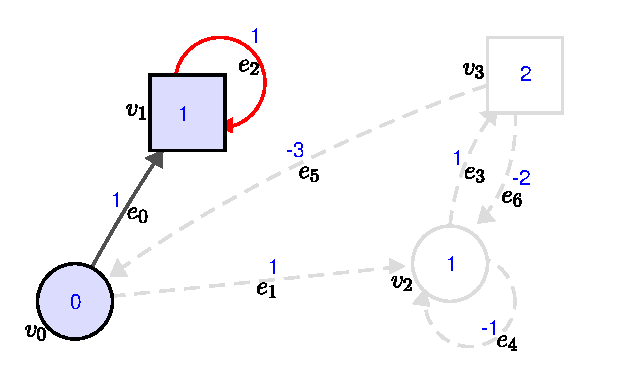
\includegraphics[width=0.8\textwidth, trim={0 0 0 0}, clip]{images/ex21.pdf}
             \vspace{-5pt} % Reduces gap between image and sub-caption
             \caption{First assignment.}
             \label{fig:ex21}
         \end{subfigure}
         \hspace{1pt} % Minimal gap
         \begin{subfigure}[t]{0.51\textwidth}
             \centering
             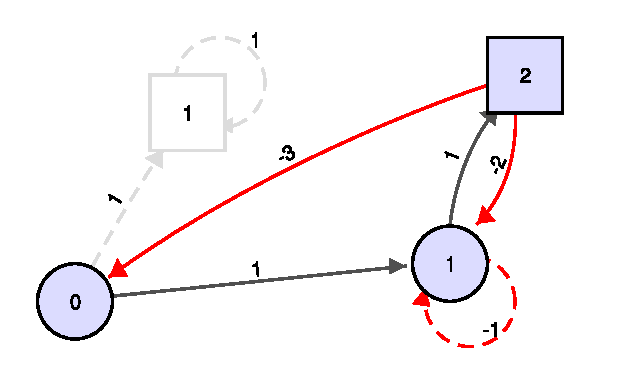
\includegraphics[width=0.8\textwidth, trim={0 0 0 0}, clip]{images/ex22.pdf}
             \vspace{-5pt}
             \caption{Second assignment}
             \label{fig:ex22}
         \end{subfigure}
     }
     \caption{The same arena as Figure~\ref{fig:ex10}, showing vertex priorities $\{0, 1, 1, 2\}$ and edge weights $\{1, 1, 1, 1, -1, -3, -2\}$.}
    \caption{The game arena from Figure~\ref{fig:ex10} annotated with vertex priorities $\Omega: V \to \{0, 1, 2\}$ and edge weights $\Xi: E \to \{-3, -2, -1, 1\}$.}
\label{fig:ex20}
\end{figure}

To illustrate the capabilities of our framework in multi-objective settings, consider the same arena operating under a combinations of conditions. We evaluate a multi-condition objective for Player~$\even$ ($\player = \even$) starting from $v_0$, requiring the simultaneous satisfaction of a Parity objective and a Positivity Energy objective ($f = f^{\omega} \land f^{\eta}$). The arena is annotated with vertex priorities $\Omega(v)$ and edge weights $\Xi(e)$ as illustrated in Figure~\ref{fig:ex20}.

The structural filtering constraints ($\mathcal{C}_{v_0}$, $\mathcal{C}_{\player}$, $\mathcal{C}_E$, and $\mathcal{C}_{\opponent}$) isolate candidate sub-graphs identically to the single-objective case, delegating the multi-objective evaluation to the global constraint $\mathcal{C}_{\noc}(f)$. In the initial search branch, the structural constraints activate $\mathcal{V}_0, \mathcal{E}_0, \mathcal{V}_1$, and $\mathcal{E}_2$ (see Figure~\ref{fig:ex21}). The global constraint evaluates the isolated self-loop from two separate dimensions:
\begin{itemize}
    \item \textbf{Cycle ($v_1 \rightarrow v_1$):} Traversing the self-loop edge $e_2$, the solver processes the joint functions:
    \[
    f^\mathcal{\omega}(v_1, v_1) = \max\{\Omega(v_1)\} \bmod 2 = 1 \bmod 2 = 1 \implies \bot,
    \]
    \[
    f^\mathcal{\eta}(v_1, v_1) = \Xi(e_2) = 1 \geq 0 \implies \top.
    \]
\end{itemize}
The global constraint computes the conjunctive victory condition $f = \bot \land \top = \bot$. Because the infinite path trapped in this sub-graph fails the Parity condition, the propagator immediately rejects the branch and forces the solver to backtrack.

In the second assignment scenario, the structural constraints isolate the alternative strategy sub-graph by activating $\mathcal{V}_0, \mathcal{E}_1, \mathcal{V}_2, \mathcal{E}_3, \mathcal{V}_3, \mathcal{E}_5$, and $\mathcal{E}_6$ (see Figure~\ref{fig:ex22}). The global constraint $\mathcal{C}_{\noc}$ extracts the two active loops and scrutinizes their infinite behaviors:
\begin{itemize}
    \item \textbf{Cycle ($v_0 \rightarrow v_2 \rightarrow v_3 \rightarrow v_0$):} Traversing edges $e_1, e_3$, and $e_5$, the solver evaluates the long loop:
    \[
    f^\mathcal{\omega}(v_0, v_2, v_3, v_0) = \max\{\Omega(v_0), \Omega(v_2), \Omega(v_3)\} \bmod 2 = \max\{0, 1, 2\} \bmod 2 = 0 \implies \top,
    \]
    \[
    f^\mathcal{\eta}(v_0, v_2, v_3, v_0) = \Xi(e_1) + \Xi(e_3) + \Xi(e_5) = 1 + 1 + (-3) = -1 < 0 \implies \bot.
    \]
    \item \textbf{Cycle ($v_2 \rightarrow v_3 \rightarrow v_2$):} Traversing the tighter internal loop via edges $e_3$ and $e_6$, the solver evaluates:
    \[
    f^\mathcal{\omega}(v_2, v_3, v_2) = \max\{\Omega(v_2), \Omega(v_3)\} \bmod 2 = \max\{1, 2\} \bmod 2 = 0 \implies \top,
    \]
    \[
    f^\mathcal{\eta}(v_2, v_3, v_2) = \Xi(e_3) + \Xi(e_6) = 1 + (-2) = -1 < 0 \implies \bot.
    \]
\end{itemize}
For both active cycles, the joint evaluation yields $f = \top \land \bot = \bot$. While this second strategy configuration successfully satisfies the Parity objective, it systematically drains the system's energy, creating loops with negative weight accumulation. 

The propagator rejects this assignment, triggering another backtrack step. Given that no alternative structural configurations remain, the solver concludes that the problem instance is unsatisfiable. Player~$\even$ possesses an Energy-winning strategy in the first sub-arena and a Parity-winning strategy in the second, but cannot satisfy both constraints simultaneously. Consequently, Player~$\even$ does not possess a winning multi-condition strategy from $v_0$.






From a theoretical perspective, it is well-established that while pure qualitative games (such as parity or Büchi) and pure quantitative games (such as energy bounds or mean-payoffs) admit optimal memoryless (positional) strategies, combining these heterogeneous objectives generally forces the players to rely on infinite or finite-memory counter-strategies to win~\cite{ChatterjeeHJ05,Chatterjee:2010}. Because our CP-based architecture maps decision variables ($\mathcal{E}$) directly to fixed, deterministic choices at each vertex, the solutions computed by our framework are strictly defined over the class of positional strategy profiles. Restricting the search space to positional configurations allows the solver to harvest the strong pruning capabilities of our global propagators while remaining highly effective for a vast array of practical synthesis and controller verification problems where memoryless implementations are preferred due to hardware constraints.


%==============================================================================

\section{Experimental Evaluation}\label{sec:experiments}

%------------------------------------------------------------------------------

\subsection{Experimental Setup and Benchmarks}\label{sec:exp_setup}

%------------------------------------------------------------------------------

\subsection{Games with Parity Games}\label{sec:exp_parity}

In this section, we evaluate the performance of \nooppc on parity games, as they represent the primary and most computationally challenging class of games for our approach. Using standard benchmarks, we assess the efficiency of \nooppc directly against state-of-the-art algorithms.

\todo{update}

For the SAT backends, we employ several high-performance solvers: \textbf{CaDiCaL} (v2.1.3) \cite{Biere:Cadical:2024}, \textbf{MiniSat} (v2.2.0) \cite{Een:MiniSat:2003}, \textbf{Kissat} (v4.0.2) \cite{Biere:Kissat:2024}, and \textbf{zChaff} (v2007.3.12) \cite{Moskewicz:zChaff:2001}. To establish a robust baseline, we compare our results with \textbf{Oink} \cite{vanDijk:2018}, which implements state-of-the-art algorithms such as Priority Promotion ($\text{PP}$ and $\text{PP+}$) and Parys' improvements ($\text{PAR}$). Additionally, we include Zielonka's Recursive Algorithm ($\text{ZRA}$) featuring the optimized attractor strategy presented in \cite{Aggarwal:2023}, which has not yet been integrated into the official Oink distribution.

The benchmarks used were taken from the PGSolver Library \cite{Friedmann:2017} and Keiren's benchmarks for parity games \cite{Keiren:2015}. The games were classified into 4 categories:

\begin{itemize}
\item \textbf{Equivalence Checking (EqC):} 69 instances from formal verification tasks ({\em e.g.}, strong and weak bisimulation), featuring complex structural connectivity typical of system architectures.
\item \textbf{Model Checking (MoC):} 90 organic benchmarks derived from $\mu$-calculus model checking, representing practical real-world verification challenges.
\item \textbf{PGSolver Collection (PGS):} 78 games taken from difficult families ({\em e.g.}, Jurdziński, ladder, and clique games~\cite{Benerecetti:2016}) used to evaluate performance against theoretical worst-case bounds of several decision procedures.
\item \textbf{Random Games (RaG):} 75 game instances with varied priority distributions, serving as a baseline for general robustness and average-case efficiency.
\end{itemize}

Furthermore, these benchmarks were partitioned into small-scale and large-scale categories based on the size of the input graphs. This distinction allows us to evaluate the feasibility of SAT-based methods on smaller instances while testing the scalability of \nooppc against dedicated solvers on larger game graphs. 

All experiments were conducted on an Intel Xeon 8260 CPU with 24 cores (non-hyperthreaded) and 268.55 GB of RAM running Linux.

\begin{table}[ht]
\centering
% \caption{Performance (in time) of Algorithms on small-scale instances  (Max vertices: EqC/MoC $\approx 10^6$, PGS/RaG $\approx 10^3$). Average time measured in seconds using PAR2 Scoring, with a max time of 60sg}

\caption{Performance of algorithms on small-scale instances (Max vertices: EqC/MoC $\approx 10^6$, PGS/RaG $\approx 10^3$). Average time is reported in seconds using PAR2 scoring with a 60s timeout.}

\setlength{\tabcolsep}{1.2mm}
{\small 
\begin{tabular}{l|rr|rr|rr|rr}
\toprule
\textbf{Algorithm} & \multicolumn{2}{c|}{\textbf{EquivalenceCh}} & \multicolumn{2}{c|}{\textbf{ModelCh}} & \multicolumn{2}{c|}{\textbf{PGSolver}} & \multicolumn{2}{c}{\textbf{RandomG}} \\
 & Time & Solved & Time & Solved & Time & Solved & Time & Solved \\
\midrule
Oink(PP)        & 0.645         & 33/33 & 0.305         & 57/57 & 0.007         & 23/23 &  0.001         & 25/25 \\
Oink(PP+)       & 0.644         & 33/33 & 0.305         & 57/57 & \textbf{0.007}& 23/23 &  0.001         & 25/25 \\
Oink(PAR)       & 0.541         & 33/33 & 0.277         & 57/57 & 0.036         & 23/23 &  0.001         & 25/25 \\
ZRA(ImpAttr)    & 0.539         & 33/33 & 0.266         & 57/57 & 0.154         & 23/23 & \textbf{0.001} & 25/25 \\
\nocq(Ours)     & \textbf{0.398}& 33/33 & \textbf{0.201}& 57/57 & 0.016         & 23/23 &  0.003         & 25/25 \\
SAT(CaDiCaL)    & 60.732        & 19/33 & 75.560        & 23/57 & 6.815         & 22/23 &  2.086         & 25/25 \\
SAT(Kissat)     & 113.050       &  2/33 & 79.001        & 21/57 & 6.064         & 22/23 &  2.628         & 25/25 \\
SAT(MiniSat)    & 79.766        & 17/33 & 79.639        & 22/57 & 6.491         & 22/23 &  2.806         & 25/25 \\
\bottomrule
\end{tabular}
}
\label{tab:paritygames-small}
\end{table}


\begin{table}[ht]
\centering
\caption{Performance of algorithms on large-scale instances (Max vertices: EqC/MoC $\approx$ 35 million, PGS/RaG $\approx 10^5$). Average time is reported in seconds using PAR2 scoring with a 60s timeout.}

\setlength{\tabcolsep}{1.2mm}
{\small 
\begin{tabular}{l|rr|rr|rr|rr}
\toprule
\textbf{Algorithm} & \multicolumn{2}{c|}{\textbf{EquivalenceCh}} & \multicolumn{2}{c|}{\textbf{ModelCh}} & \multicolumn{2}{c|}{\textbf{PGSolver}} & \multicolumn{2}{c}{\textbf{RandomG}} \\
 & Time & Solved & Time & Solved & Time & Solved & Time & Solved \\
\midrule
Oink(PP)        & 29.375         & 30/36 & 9.003         & 33/33 & 8.369         & 50/55 & 0.039         & 50/50 \\
Oink(PP+)       & 29.392         & 30/36 & 8.986         & 33/33 & 8.371         & 50/55 & \textbf{0.039}& 50/50 \\
Oink(PAR)       & 28.525         & 30/36 & 8.345         & 33/33 & 16.798        & 43/55 & 0.043        & 50/50 \\
ZRA(ImpAttr)    & 21.249         & 35/36 & 8.606         & 33/33 & 16.632        & 43/55 & 0.042         & 50/50 \\
\nocq(Ours)     & \textbf{13.502}& 36/36 & \textbf{3.838}& 33/33 & \textbf{5.659}& 54/55 & 0.081         & 50/50 \\
\bottomrule
\end{tabular}
}
\label{tab:paritygames-large}
\end{table}

Table~\ref{tab:paritygames-small} presents a consolidated performance comparison on small-scale instances. In this setting, \nocq outperforms traditional SAT-based approaches by up to three orders of magnitude in execution time while achieving 100\% coverage (compared to the low timeout-heavy completion rates of SAT solvers). Furthermore, \nocq outperforms specialized parity game solvers on the \texttt{EquivalenceCh} and \texttt{ModelCh} benchmarks by 25\% to 35\%, while remaining highly competitive on the remaining families—differing only by a marginal fraction of a second.

For large-scale instances, as shown in Table~\ref{tab:paritygames-large}, standard SAT-based approaches are omitted due to their inability to scale within reasonable resource limits. In this challenging context, \nocq demonstrates superior robustness and scalability, consistently outperforming specialized solvers in both execution time and instance coverage. On \texttt{EquivalenceCh} and \texttt{ModelCh}, \nocq achieves the fastest runtimes, delivering speedups of up to $2\times$ over the next best algorithms while maintaining 100\% coverage. Crucially, on the structured \texttt{PGSolver} collection, \nocq solves the highest number of instances (54/55)—significantly outperforming ZRA (43/55) and the Oink variants (50/55) while cutting execution times by up to 66\%. While the Oink variants remain nominally faster on \texttt{RandomG}, the absolute difference is a marginal fraction of a second, highlighting \nocq's effectiveness as a highly robust, general-purpose solver for large-scale parity games.

%------------------------------------------------------------------------------

\subsection{Qualitative and Quantitative Goals and Formal Verification}\label{sec:exp_quantitative}

\todo{update}

One of \nocq's main features is the ability to handle quantitative goals within the same CP-based framework. 
%
\nocq implements a core algorithm designed to compute positional strategies, which are optimal in case only qualitative (parity) or only quantitative goals are given. However, when combined, positional strategies may no longer be optimal~\cite{ChatterjeeHJ05,Chatterjee:2010}. As such, the solutions that \nocq computes are for games where only positional strategies are allowed. 
%
In this context, the next set of benchmarks demonstrates \nocq's performance when solving such kinds of games when enriched with additional quantitative (energy and/or mean-payoff) requirements.  
%
To this end, first, we used the same games of Section \ref{sec:exp_parity} but now added with random weights over the edges using a fair distribution between -1,000 and 1,000. These benchmarks utilize random positional vertex assignments and randomly generated thresholds. We assess the tool's efficiency across various multi-objective configurations defined by the winning condition $\gamma_{p} = \omega \otimes \eta \otimes \mu$, where $\otimes$ denotes the product composition of parity ($\omega$), energy ($\eta$), and mean-payoff ($\mu$) objectives.

\begin{table}[ht]
\centering
\caption{Performance of \nocq with different winning conditions on small and large-scale instances on specialized families of Games. Same configuration as Table \ref{tab:paritygames-large}.}
\setlength{\tabcolsep}{1.2mm}
{\small 
\begin{tabular}{l|rr|rr|rr|rr}
\toprule
\textbf{Algorithm} & \multicolumn{2}{c|}{\textbf{EquivalenceCh}} & \multicolumn{2}{c|}{\textbf{ModelCh}} & \multicolumn{2}{c|}{\textbf{PGSolver}} & \multicolumn{2}{c}{\textbf{RandomG}} \\
 & Time & Solved & Time & Solved & Time & Solved & Time & Solved \\
\midrule
\textbf{$\omega$}
    & 6.950  & 69/69 & 2.019 & 90/90 & 2.838  & 78/78 & 0.042  & 75/75 \\
\textbf{$\eta$}
    & 21.272 & 57/69 & 2.019 & 90/90 & 6.371  & 74/78 & 1.671  & 74/75 \\
\textbf{$\mu$}
    & 21.271 & 57/69 & 2.019 & 90/90 & 13.568 & 70/78 & 30.990 & 56/75 \\
\textbf{$\omega \otimes \eta$}
    & 21.272 & 57/69 & 2.021 & 90/90 & 6.391  & 74/78 & 1.669  & 74/75 \\
\textbf{$\omega \otimes \mu$}
    & 21.274 & 57/69 & 2.019 & 90/90 & 11.126 & 71/78 & 21.066 & 62/75 \\
\textbf{$\eta \otimes \mu$}
    & 21.271 & 57/69 & 2.021 & 90/90 & 8.044  & 73/78 & 16.079 & 65/75 \\
\textbf{$\omega \otimes \eta \otimes \mu$}
    & 23.010 & 56/69 & 2.019 & 90/90 & 10.685 & 72/78 & 22.457 & 61/75 \\
\bottomrule
\end{tabular}
}
\label{tab:quantitative-benchmarks}
\end{table}

Table~\ref{tab:quantitative-benchmarks} shows that while the baseline condition~$\omega$ consistently achieves a 100\% solving rate and minimal execution times across all datasets, the introduction of~$\eta$ and~$\mu$ imposes distinct computational overheads, with~$\mu$ acting as the primary bottleneck for performance degradation and timeouts. This complexity is highly dependent on graph structure: while the large-scale \texttt{Model Checking} instances remain entirely unaffected by condition complexity due to structural properties that neutralize evaluation overhead, chaotic environments like \texttt{Random Games} show extreme sensitivity, causing pure~$\mu$ to drop to 56/75 solved instances. Interestingly, the data reveals a beneficial constraint interaction where combining~$\mu$ with~$\omega$ or~$\eta$ (such as in~$\eta \otimes \mu$) frequently mitigates this overhead, improving runtimes and solving more instances than~$\mu$ alone by effectively pruning the search space.

Second, we evaluated a selection of random benchmarks as proposed by~\cite{Chaloupka:2011}, which follow the design of the \texttt{SPRAND} generator~\cite{CherkasskyBoris:1996} for energy and mean-payoff games. These benchmarks are categorized by their structural properties using the naming convention \texttt{R\_<d><s\_key>} introduced in~\cite{Chaloupka:2011}, where \texttt{<d>} represents the vertex out-degree (density) and \texttt{<s\_key>} denotes the state-space size. For this benchmarking suite, we consider a high density of $10$ outgoing edges per vertex. The vertex counts scale according to the criteria and labeling defined in~\cite{Chaloupka:2011}: $b = 2^{17}$ and $h = 2^{18}$. Furthermore, we extended the evaluation to larger games by introducing two additional scales: $xb = 2^{19}$ and $xh = 2^{20}$, while broadening the edge weight range to approximately $\pm 10^4$ (from $-10,000$ to $10,000$).

\begin{table}[ht]
\centering
\caption{Performance of \nocq with different winning conditions on random instances with SPRAND structure \cite{Chaloupka:2011}. Same configuration as Table \ref{tab:quantitative-benchmarks}.}
\setlength{\tabcolsep}{1.2mm}
{\small 
\begin{tabular}{l|rr|rr|rr|rr}
\toprule
\textbf{Conditions} & \multicolumn{2}{c|}{\textbf{R\_10b}} & \multicolumn{2}{c|}{\textbf{R\_10h}} & \multicolumn{2}{c|}{\textbf{R\_10xb}} & \multicolumn{2}{c}{\textbf{R\_10xh}} \\
& Time & Solved & Time & Solved & Time & Solved & Time & Solved \\
\midrule
\textbf{$\omega$}
    &  0.201 & 30/30 &  0.456 & 30/30 &  1.046 & 30/30 &  2.137 & 30/30 \\
\textbf{$\eta$}
    & 30.721 & 23/30 & 37.617 & 21/30 & 26.367 & 24/30 & 38.197 & 21/30 \\
\textbf{$\mu$}
    & 40.134 & 20/30 & 52.263 & 17/30 & 52.568 & 17/30 & 37.439 & 21/30 \\
\textbf{$\omega \otimes \eta$}
    & 31.389 & 23/30 & 23.013 & 25/30 &  6.674 & 29/30 & 10.722 & 28/30 \\
\textbf{$\omega \otimes \mu$}
    & 36.139 & 21/30 & 52.254 & 17/30 & 56.530 & 16/30 & 37.405 & 21/30 \\
\textbf{$\eta \otimes \mu$}
    & 40.130 & 20/30 & 52.258 & 17/30 & 56.528 & 16/30 & 37.383 & 21/30 \\
\textbf{$\omega \otimes \eta \otimes \mu$}
    & 40.129 & 20/30 & 52.258 & 17/30 & 56.515 & 16/30 & 37.375 & 21/30 \\
\bottomrule
\end{tabular}
}
\label{tab:quantitative-chpk}
\end{table}

The results in Table~\ref{tab:quantitative-chpk} are highly consistent with the trends observed in Table~\ref{tab:quantitative-benchmarks}, confirming that the composition of winning conditions does not inherently compound computational difficulty. The baseline condition~$\omega$ scale exceptionally well across the high-density random benchmarks, maintaining a 100\% solving rate (30/30) and completing in under 2.2 seconds even on the largest $R\_10xh$ instances.

A key strength of the \nocq toolchain is highlighted in the multi-objective configurations. When combining parity with an energy objective (e.g., $\omega \otimes \eta$), the solver frequently demonstrates a pruning effect, where the parity condition helps narrow the search space, leading to more robust solving times compared to other combinations. However, for the most complex triple-objective configurations ($\omega \otimes \eta \otimes \mu$), the performance tends to be bottlenecked by the mean-payoff component.

Since the benchmarking software in \cite{Chaloupka:2011} has not been released, we could not perform a side-by-side comparison. Nevertheless, our results for energy games show a reasonable solving time compared with their reported results.  Furthermore, obtaining standardized benchmarks for this class of games remains a challenge, as few publicly available datasets or implementations exist.

%==============================================================================

\section{Improving Constraint base model}\label{sec:improved_cp}

%------------------------------------------------------------------------------

\subsection{Improved Filtering Strategy via Memoization (\nocmemo)}\label{sec:nocmemo}

To avoid the potential path explosion of the \noceager while retaining predictive pruning, we introduce a bounded variant that tracks previously analyzed cycles through an internal memoization layer.
%
To do so, one can use Algorithm \ref{alg:nocmemo}, which incorporates a parameter $\textit{mem}$ that stores, for each edge: the starting node of an infinite path and the associated $f$ outcome. This information is updated whenever a cycle is found (line~\ref{alg:nocmemo:findcycle1}). If $\textit{mem}$ does not contain information about the next edge $e'$, or a new better $f$ outcome was found, then the propagator proceeds recursively as before (lines~\ref{alg:nocmemo:check1} and \ref{alg:nocmemo:check2}). Otherwise, it uses the stored information for the new edge (line~\ref{alg:nocmemo:update2}).

This generalization results in a bounded worst-case runtime, as the recursion is strictly limited by the number of graph edges and the capacity of the domain governing the winning condition. An edge triggers a recursive look-ahead re-evaluation only when a strictly more dominant property is encountered, meaning the maximum number of updates per edge is directly bounded by the number of distinct values the dominant property can assume.

While this mechanism enforces a strict bound on execution relative to the size of the property's domain, the underlying complexity classification varies by winning condition. For standard qualitative conditions like Büchi and Parity, the domain scales polynomially with the graph size and priorities. For quantitative, weight-based conditions such as Energy and Mean-Payoff, the domain size depends on the maximum absolute edge weight, resulting in a pseudo-polynomial worst-case bound rather than a purely polynomial one.

Furthermore, because the memoization only captures cycles sharing the exact same starting node, the propagator remains incomplete and may miss cycles that cross paths globally. To preserve full completeness across all supported winning conditions, \nocmemo should be used in conjunction with the global \nocchecker.

\begin{algorithm}[htb]
\caption{\textbf{\nocmemo}}
\small
\textbf{Input}: $path_V, path_E, v, e, \mathcal{X}, \textit{defined}, \textit{mem}$ \\
\textbf{Output}: $\top$ if look-ahead is valid; $\bot$ if a fatal conflict occurs
\begin{algorithmic}[1]
    \IF{$v \in path_V$} \label{alg:nocmemo:pathcheck}
        \STATE $i_v \gets$ \textit{find}$(v,\ path_V)$ \label{alg:nocmemo:findcycle1}
        \STATE $d \gets \text{evaluate dominant property along } path_V[i_v:]$
        \STATE $\textit{mem}[e] \gets (v,\ d)$ \label{alg:nocmemo:update1}
        \IF{$\neg f(path_V[i_v:])$} \label{alg:nocmemo:checkopponent}
            \STATE $\textit{reason} \gets \textit{clausify}(\neg path_E)$ \label{alg:nocmemo:reason}
            \STATE \textbf{if }not ($\mathcal{E}_e \gets (\bot, \textit{reason}))$ \textbf{then return $\bot$}
        \ENDIF
    \ELSIF{$\textit{defined}$} \label{alg:nocmemo:defcheck}
        \FOR{$e' \in \textit{edges}(v)\ \textbf{where}\ \mathcal{E}_{e'} \ne \bot$}
            \STATE $(v_{mem},\ d_{mem}) \gets \textit{mem}[e']$
            \STATE $p_V \gets path_V \cup \{v\}$
            \STATE $p_E \gets path_E \cup \{e'\}$
            \STATE $w \gets \textit{target}(e')$
            \STATE $\textit{def} \gets (\mathcal{E}_{e'} = \top)$
 
            \IF{$(v_{mem}, d_{mem}) = (\text{null}, \text{null})$}
                \STATE \nocmemo($p_V, p_E, w, e', \mathcal{X}, \textit{def}, \textit{mem}$)\label{alg:nocmemo:check1}
            \ELSE
                \STATE $i_v \gets \textit{find}(v_{mem},\ path_V)$ \label{alg:nocmemo:findcycle2}
                \STATE $d \gets \text{evaluate property along } path_V[i_v:]$
                \IF{$v_{mem} \in path_V \land d \text{ dominates } d_{mem} \text{ under criteria } f$}
                    \STATE \nocmemo($p_V, p_E, w, e', \mathcal{X}, \textit{def}, \textit{mem}$)\label{alg:nocmemo:check2}
                \ELSE
                    \STATE $\textit{mem}[e] \gets \textit{mem}[e']$ \label{alg:nocmemo:update2}
                \ENDIF
            \ENDIF
        \ENDFOR
    \ENDIF
    \RETURN $\top$
\end{algorithmic}
\label{alg:nocmemo}
\end{algorithm}

%------------------------------------------------------------------------------

\subsection{The Integer Formulation (\nooppc-Int)}\label{sec:noc_int}

%------------------------------------------------------------------------------

\subsection{Search Strategies and Game-Specific Heuristics}\label{sec:search_heuristics}

%------------------------------------------------------------------------------

\subsection{Experimental Analysis of Improvements}\label{sec:improve_experiments}

%==============================================================================

\section{Conclusions and Future Work}\label{sec:conclusion}

% To print the credit authorship contribution details
\printcredits

\newpage

%% Loading bibliography style file
%\bibliographystyle{model1-num-names}
\bibliographystyle{cas-model2-names}

% Loading bibliography database
\bibliography{paper}

% Biography
%\bio{}
% Here goes the biography details.
%\endbio

%\bio{pic1}
% Here goes the biography details.
%\endbio

\end{document}

